\section{Processing methods}
Looking at the challenges presented in the previous section it is obvious that there are numerous factors, in which the existing state-of-the-art systems for capacitive sensing can be improved. 
\subsection{Sparsely distributed sensor arrays}
Sparsely distributed sensor arrays refer to layouts that limit the number of available sensors either by environmental parameters or by design. 
\subsubsection{3D location tracking}
 \begin{figure}[h]
\centering
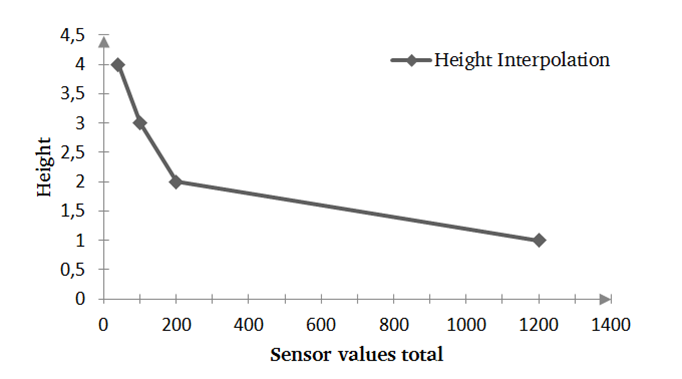
\includegraphics[width=0.6\textwidth]{images/magicbox_data_zaxis}
\caption{Piecewise linear hand distance estimation \cite{Braun2011MultiInputDevice}}
\label{fig:magicbox_data_zaxis}
\end{figure}
%Figure 29 Piecewise linear hand distance estimation [78]
The first data processing step of the MagicBox is the planar localization of the hand, following the weighted average algorithm previously presented. In order to calculate the distance of the hand from the plane we are using a piecewise linear interpolation, that resembles the response curve of a single sensor \cite{Braun2011MultiInputDevice}.
\begin{figure}[h]
\centering
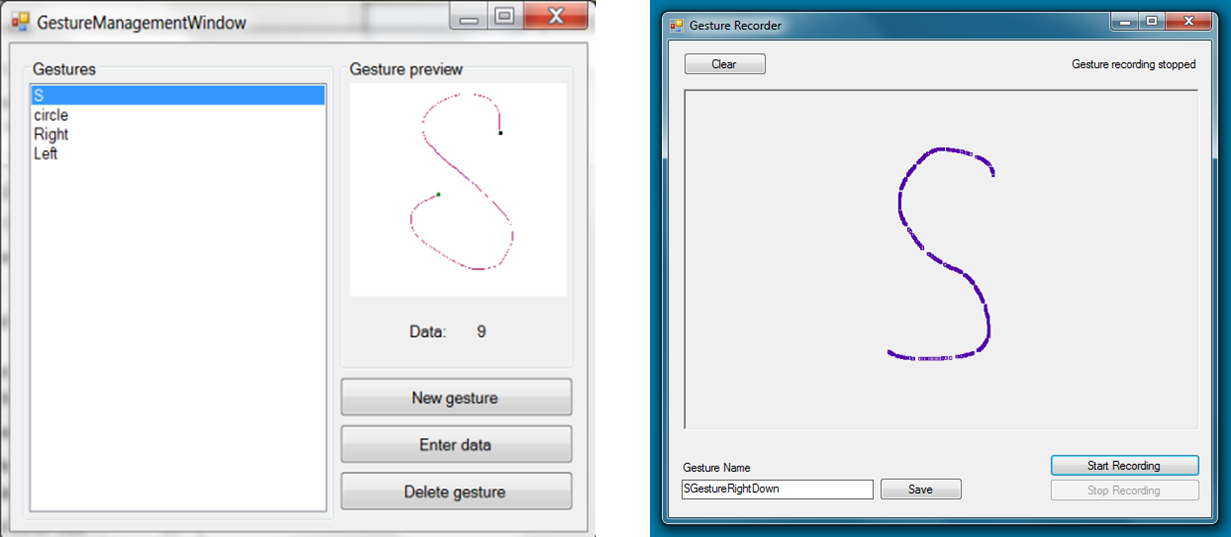
\includegraphics[width=0.7\textwidth]{images/magicbox_data_gest}
\caption{Gesture overview module (left) and gesture recorder (right)}
\label{fig:magicbox_data_gest}
\end{figure}
%Figure 30 Gesture overview module (left) and gesture recorder (right)
An addition of the MagicBox was a generic gesture recognition module based on methods similar to mouse gesture recognition \cite{braun2013capacitive}, albeit adapted for three dimensional locations. The developed debug software allows defining an arbitrary set of potential gestures and adding training data, as shown in Figure \ref{fig:magicbox_data_gest}. The module is looking for matches based on the most recent set of locations. 
\subsubsection{Large-area location tracking}
Using long wire electrodes may result in considerable noise and influence from outside electric fields. Therefore CapFloor requires preprocessing to reduce the noise and achieve a more robust high-level data processing. The localization uses the weighted average algorithm that has been presented previously. 
\begin{figure}[h]
\centering
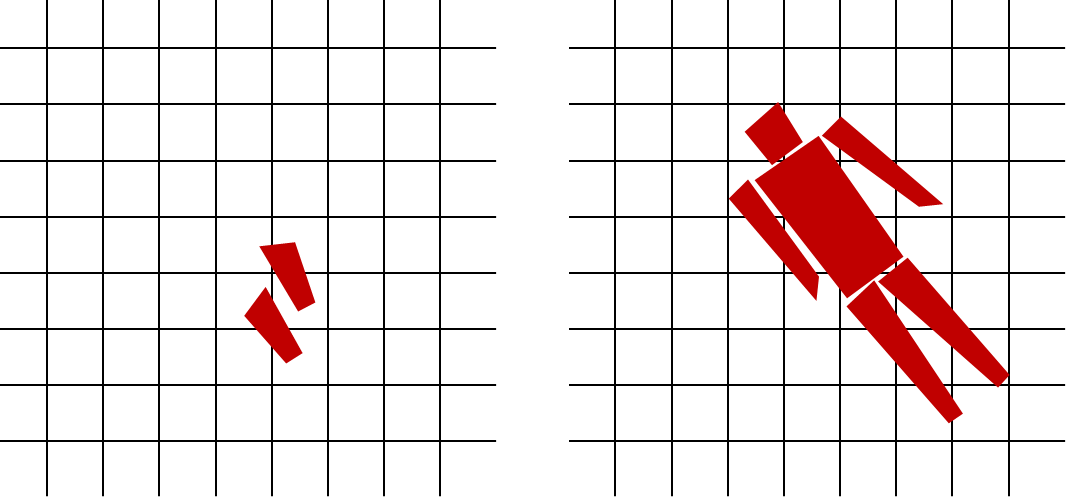
\includegraphics[width=0.8\textwidth]{images/floor_shapes}
\caption{Shapes of a standing and lynig person on top of the CapFloor grid}
\label{fig:capfloor_shapes}
\end{figure}
The fall detection is using a time-series analysis of the aggregated values of the sensors that are currently detecting an object. This method is using the assumption that the overall sensor response is roughly equivalent to the shape of the object that is closest to the surface, resulting in a higher capacitance of the overall system, similar to the plate capacitor model. This effect is shown in Figure \ref{fig:capfloor_shapes}. The sum $s$ of all n sensor values $r$ is the closest equivalent to the system capacitance and therefore a viable measure. If the overall value is beyond a certain threshold $v_l$ we can consider a lying person $p_l$.
\begin{equation}
s=\sum^n_{i=0}{r_i}\ \ \ ,\ \ \ p_l=\left\{ \begin{array}{c}
1,\ \ \ s\ge v_l \\ 
0,\ \ \ s<v_l \end{array}
\right.
\end{equation}
In order to increase the robustness this threshold has to be exceeded for a certain amount of time $t_m$. In consequence a fall $f$ is detected if the following equation is 1.
\begin{equation}
f=\prod^{t_m}_{j=0}{p_{l,t_j}}
\end{equation}
\subsection{Model-driven fitting methods}
\subsubsection{Single-body models}
\begin{figure}[h]
\centering
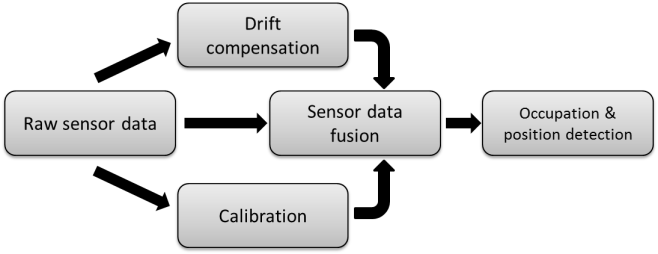
\includegraphics[width=0.7\textwidth]{images/smartbed_proc}
\caption{Data processing components \cite{braun2012context}}
\label{fig:smartbed_proc}
\end{figure}
The different components of the Smart Bed data processing are shown in Figure \ref{fig:smartbed_proc}. Raw sensor data is distributed to three different modules, the calibration which is determining the initial parameters for the sensor data fusion, the drift compensation that alters those parameters according to long term trends and finally the sensor data fusion module that processes the data and does feed it to the occupation \& position detection. Calibration and drift compensation follow the previously presented model \cite{braun2012context}. 
\begin{figure}[h]
\centering
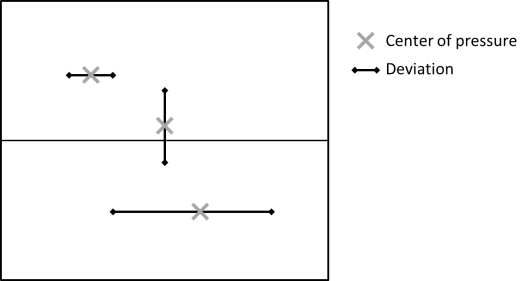
\includegraphics[width=0.7\textwidth]{images/smartbed_cog}
\caption{Calculating centers of pressures and deviation \cite{braun2012context}}
\label{fig:smartbed_cog}
\end{figure}
Occupation and position detection is performed by dividing the two person bed into left and right and individually calculating for each side the total sensor values, assumed center of pressure using weighted average and the standard deviation (Figure \ref{fig:smartbed_cog}). The same calculation is done between the two sides to distinguish where is activity or if one person is lying diagonally.
Using these six intermediate values we can now map various poses. If all activity is on one side and the horizontal deviation is low, we can assume that one person is sitting. We can additionally use the intermediate values to calculate more information, e.g. the exact location a person is sitting at. 
The data processing for the sleep phase recognition is based on detecting the sensor data variations in order to analyze movement. Discriminating between sleep phases using movement is a common approach that has been used in the past \cite{salmi86}. Using a sparse set of sensors it is possible to detect movement by comparing subsequent sensor readings and associate it to different sleep phases using different activity profiles. The system is based on the same prototype as the posture recognition system \cite{Djakow2013movibed}.
\subsubsection{Multi-body models}
\begin{figure}[h]
\centering
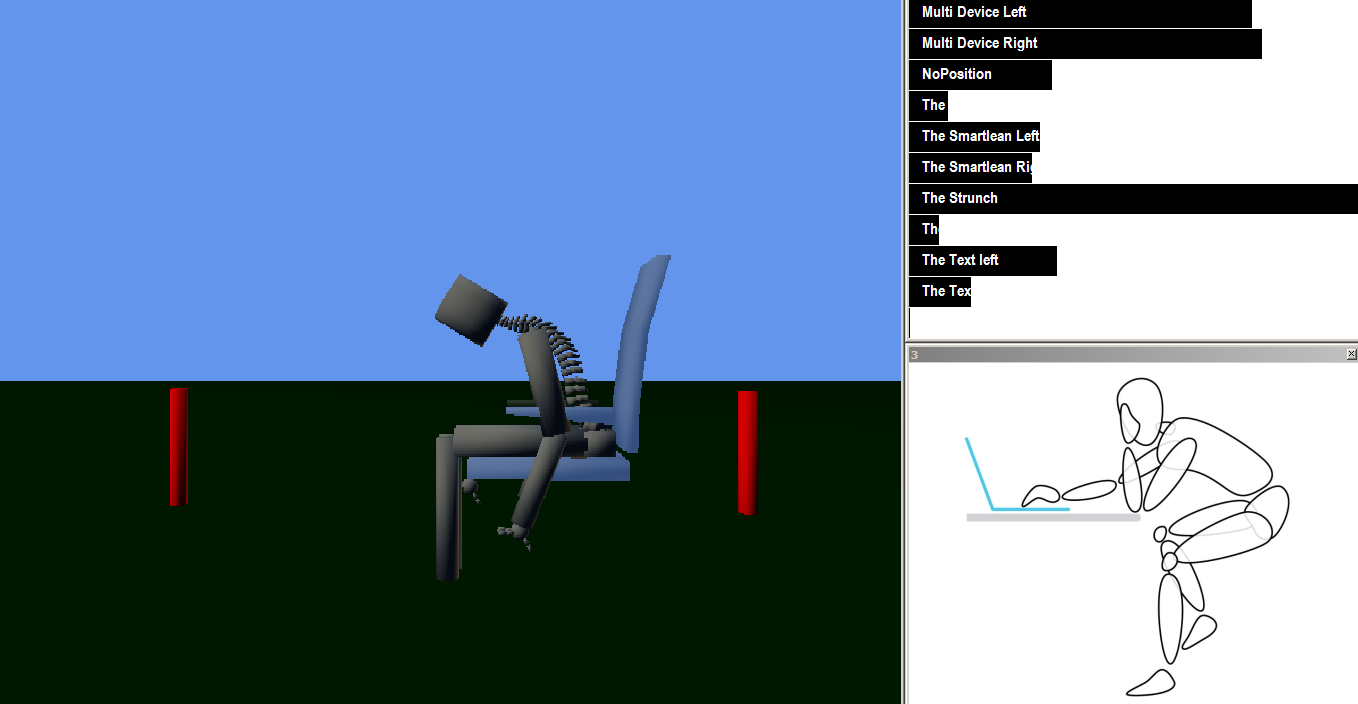
\includegraphics[width=0.7\textwidth]{images/smartchair_software}
\caption{Screenshot of the Capacitive Chair application showing the fitted 3D model on the left, posture detection on the upper right and the recognized posture on the lower right}
\label{fig:smartchair_software}
\end{figure}
In Figure \ref{fig:smartchair_software} we can see a screenshot of the Capacitive Chair debug application. On the left side we see a 3D model that is fitted to a chair model according to the current sensor values, in the middle the results of the machine learning module and the recognized posture and on the right side the currently running breathing rate detection as both Fourier analysis and signal deviation analysis.
All processing methods work on filtered and normalized sensor data. The difference in shape, material and size of the electrodes necessitates slight adaptations to noise filtering and data processing. As an example only the conductive thread backrest electrode is used in the breathing rate detection. 
The 3D model is using a simplified human joint model comprised of 13 connected components. Based on the current sensor readings, single parts or groups of components are fitted to the virtual chair. The process is a mix of posture mapping as found in the smart bed and modification of the dynamic links between the single components \cite{Braun2013ChairAid}.
\begin{figure}[h]
\centering
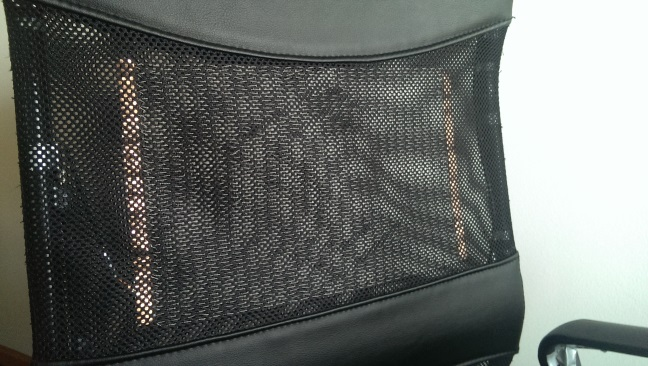
\includegraphics[width=0.7\textwidth]{images/smartchair_thread}
\caption{Screenshot of the Capacitive Chair application showing the fitted 3D model on the left, posture detection on the upper right and the recognized posture on the lower right}
\label{fig:smartchair_thread}
\end{figure}
We use a simple RBF neural network and training data collected by two different persons to match the input from eight sensors to nine potential output postures that are associated to different working situations. An early observation is that certain postures are difficult to distinguish given the limited number of sensors and the similarity of the postures on the rigid chair. Either a higher number of sensors or a more versatile chair could be used that allows gathering additional information required to distinguish the different poses more reliably. 

The breathing rate detection is operating on a single electrode that is integrated into a mesh on the backrest using conductive thread. The setup is shown in Figure \ref{fig:smartchair_thread}. Consequently the surface of the electrode is large and able to pick up the chest movement. Two different methods of data processing are used and fused to get the final breathing rate. Using a fast Fourier transformation the signal is transformed into the frequency space. We are looking for significant signal portions in frequency areas that can be associated to breathing, between $0.2Hz$ and $10Hz$. The second method is to look for zero-crossings of the sensor signal through an adaptive baseline. If a person is breathing in the sensor value will decrease resulting in the signal dropping below the long-term average, and rise above when the person is breathing out. Accordingly the breathing rate can be calculated by counting the zero-crossings.
\subsection{Heterogeneous sensor systems}
\subsubsection{Heterogeneous capacitive arrays}
\begin{figure}[h]
\centering
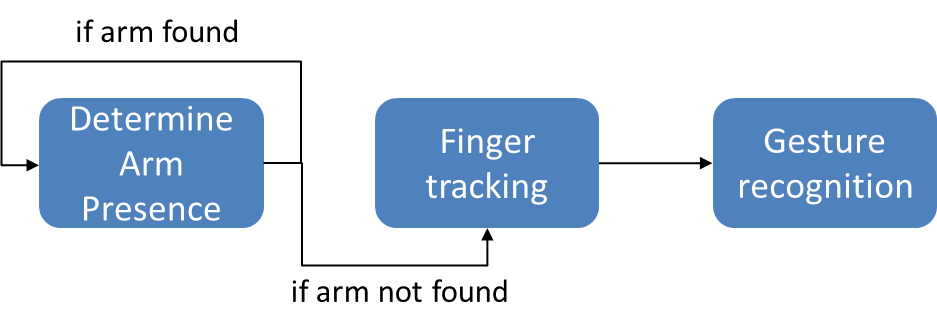
\includegraphics[width=0.4\textwidth]{images/armrest_dataproc}
\caption{Data processing pipeline of Active Armrest}
\label{fig:armrest_dataproc}
\end{figure}
%Figure 25 Data processing pipeline of Active Armrest
As we already mentioned, the Active Armrest electrodes are put into two groups. The data processing for both groups is distinctly different. In order to detect the presence of the arm using the two-electrode group a simple threshold on the accumulated values is used. The six sensor array in the front (touch area) is using the presented weighted average method to calculate finger positions. Additionally a threshold is used to distinguish one and two fingers. Overall there is a data processing pipeline as shown in Figure \ref{fig:armrest_proto}. The finger tracking and gesture recognition will be inactive until it is ensured that no arm is present. 

\subsubsection{Heterogeneous sensor fusion}
\begin{figure}[h]
\centering
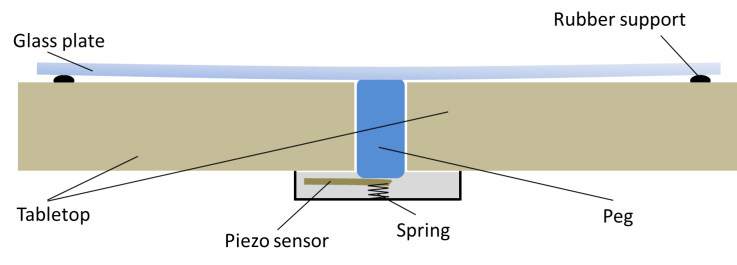
\includegraphics[width=0.7\textwidth]{images/captap_peg}
\caption{Suspended peg knock detection system for CapTap \cite{Braun2013ChairAid}}
\label{fig:captap_peg}
\end{figure}
%Figure 34 Suspended peg knock detection system for CapTap [80]
The hand location of the CapTap is similar to the methods presented for the MagicBox. We add the additional component of knock detection to provide selection events when touching the surface. Figure \ref{fig:captap_sketch} shows a sketch of the knock detection system. The table has a glass plate that is suspended on some rubber supports. In the center of the table we attach a small peg (enlarged in sketch) that creates a connection between the glass plate and a piezo sensor. If the glass plate starts vibrating from a touch we can measure this using the piezo sensor \cite{Braun2013ChairAid}. If a notable vibration is measured we are collecting the next 50 samples, resulting in a window of 250 milliseconds. To distinguish single and double knocks we calculate the weighted average within this window to get a measure for the distribution of sensor values within. If the average is closer to the beginning of the window the resulting event should be a single knock, and a double if the average is closer to the end of the window.
Hand localization and knock detection are working independently and are combined later in the software. It is reasonable to combine this, e.g. to ignore knock events that are occurring without a hand present. They may be indicative of a person doing a strong step close to the table.

\subsection{Image-based processing}
Their ability to detect changes in the electric field over a distance has led to capacitive proximity being regarded as similar to cameras. Smith et al. consequently called their approach electric field imaging, as particularly shunt mode measurements and their constrained electric fields allow applying certain image processing methods, e.g. tomography \cite{Smith1999a}. They were critical of using similar methods for shunt mode, noting the following statement.
\begin{quote}
Loading mode measurements can be likened
to images formed without a lens, since only one "end" of
each field line is constrained by the measurement. \cite{smith1998electric}
\end{quote}
Nonetheless, loading mode has certain advantages, particularly if all electrodes are in a single plane and we would like to have a higher sensitivity at a distance from the plane it is advantageous if there is no receiving potential nearby. One example for this planar electrode setup is large area gesture interaction devices, e.g. a table that is able to track the position of arms and hands in three dimensions. There is a plethora of image-based object detection and tracking algorithms that can be also used for capacitive proximity sensor data processing. There is a short process that I propose to realize this arm and hand tracking that includes some general steps that can be used to identify a variety of objects. The process is distinguished into four distinct steps:
\begin{itemize}
\item Creating a grayscale image from the acquired sensor data
\item Apply a feature-preserving image upscaling method
\item Find the contours of the present objects according to pixel values
\item Analyze the image moments of the contour areas and fit human arms
\end{itemize} 

\begin{figure}[h]
\centering

\includegraphics[width=0.5\textwidth]{images/proc_im_pixels}
\caption{Pixel array mapped from sensor values}
\label{fig:proc_im_pixels}
\end{figure}

The most challenging aspect of the first step is the low resolution of a reconstructed image. In order to achieve a mid-range distance resolution that allows detecting objects within 30 or 40 cm it is necessary to use electrodes that are sufficiently large. Thus, an example device uses an array of 6x4 sensor electrodes, resulting in an image of only 24 pixels. Typically the sensor values are an integer value in a range between 0 and 15000. Accordingly we can create a single-channel image with a channel depth of two bytes. In our case we use a linear mapping of sensor values to pixel intensities. An exemplary result image of this mapping is shown in \ref{fig:proc_im_pixels} (with enlarged pixels). In this format it is difficult to gather information about the exact position of the arms and thus we need to apply further processing before finding the contours and fitting arm objects.
\begin{figure}[h]
\centering
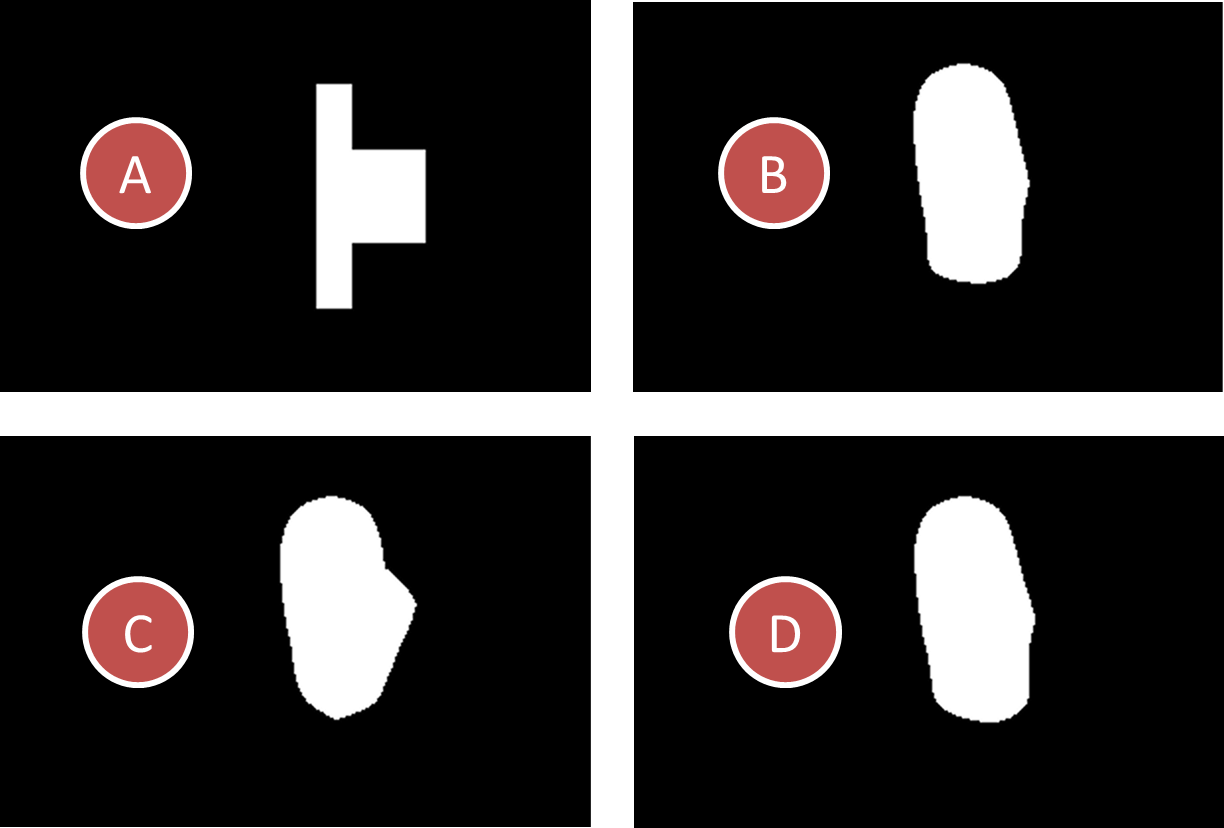
\includegraphics[width=0.9\textwidth]{images/proc_im_interpol}
\caption{Effect of different upscaling methods on shape, (A) nearest neighbor, (B) bicubic, (C) bilinear, (D) Lanczos4 - shown as thresholded binary images (pixel intensity > 30)}
\label{fig:proc_im_interpol}
\end{figure}

\subsubsection{Acquire and optimize contours}
In order to get the relevant contours of objects in the interaction area we have to apply some further processing. The first step is to enlarge the image using a feature-preserving scaling method. As all sensors are prone to environmental noise we apply some thresholding based on the pixel intensities before looking for contours. The result is an enlarged binary image of black and white pixels. We have tested four different image scaling methods, nearest neighbor, bilinear interpolation, bicubic interpolation and Lanczos interpolation. Exemplary results are shown in \ref{fig:proc_im_interpol}. The Lanczos interpolation showed the best results but is most processing intensive. However, since we are dealing with small images it is reasonable for CapTap. The contours are calculated based on those binary images, defined as the borders between black and white regions. For further processing we are looking into the distribution and the intensities of the pixels within the specified region.
\begin{figure}[h]
\centering
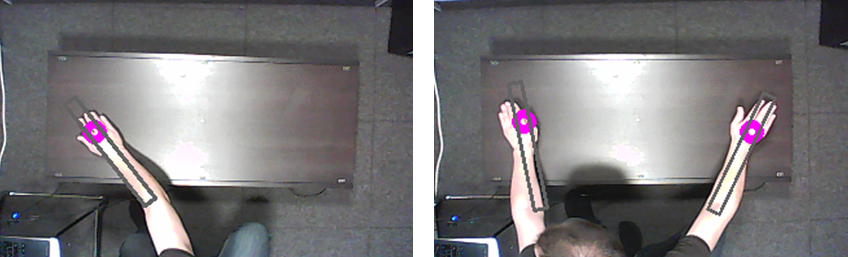
\includegraphics[width=0.9\textwidth]{images/proc_im_arms}
\caption{Overhead camera picture of the scene overlaid with live arm and palm reconstruction for one arm (left) and two arms (right)}
\label{fig:proc_im_arms}
\end{figure}

\subsubsection{Palm and arm fitting}
The last step of identifying and tracking the arms is to fit the position and orientation of the palms and arm into the acquired object contours. For this task we are analyzing the image moments within the contours. These are certain particular weighted averages of pixel intensities, or a function thereof \cite{hu1962visual}. They can be calculated using the following equation, whereas $j$ and $i$ define the order and $I(x,y)$ is the pixel intensity at a given position. We can use this to calculate the center point $(\overline{x},\overline{y})$, leading to the central moments $mu_ji$ that are required to determine the orientation of the contour as angle $\gamma$.
%m_ji=∑_(x,y)▒〖I(x,y) x^j y^i  〗,x ̅=m_10/m_00 ,y ̅=m_01/m_00 
%〖mu〗_ji=∑_(x,y)▒〖I(x,y) (x-x ̅ )^j (y-y ̅ )^i  〗
% γ=0.5∙arctan (2∙〖mu〗_11)/(〖mu〗_20-〖mu〗_02 )
\begin{equation}
m_ji=\sum_{(x,y)}{I(x,y)x^jy^i}
\end{equation}
\begin{equation}
\overline{x}=\frac{m_10}{m_00}, \overline{y}=\frac{m_01}{m_00}
\end{equation}
\begin{equation}
mu_{ji}=\sum_{(x,y)}{I(x,y)(x-\overline{x})^j(y-\overline{y})^i}
\end{equation}
\begin{equation}
\gamma=0.5\cdot arctan\frac{2\cdot{mu_{11}}}{mu_{20}-mu_{02}}
\end{equation}
 
We use the center point and orientation to calculate the estimated position of the palm of the hands. These points are the basis for the subsequent gesture recognition. Additionally, we are using separate Kalman filters for smoothing the different palm positions and arm orientation. The resulting arm reconstruction and the actual arm position in a photo are shown in \ref{fig:proc_im_arms}. We installed a simple webcam above the table and registered the table position to the camera image. 

The arm reconstruction so far is mostly used to determine the arm position. Another potential use of the arm orientation is to improve the merging of two hands. While the system can't distinguish from a single sensor if one hand is close or two hands are further away, we can use the presence of two arms to identify the overall number of objects in the detection range. 
\subsubsection{Intensity-based elevation estimate}
A distinct challenge of the capacitive hand tracking is the considerable directional difference in available resolution. While we can use the presented image analysis to track the planar position of the arms over the whole table area of 80cm width and 50cm depth, estimating the elevation of the arm above the table is restricted by the proximity range of the single sensor. Typically the achievable range maxes out at around 35cm, depending on environmental conditions. In a plate capacitor system the distance $d$ is proportional according to size of the plates $A$ and resulting capacitance $C$. Due to the linear mapping of sensor capacitance measurements to pixel intensities $I$ we can use the image moment within a contour $S$ as estimate of the actual capacitance, and calculate the elevation $e$ according to the following equations:

\begin{align}
d&\propto{\tfrac{C}{A}} & S&\propto{\tfrac{m_{00}}{\int{S}}}
\end{align}

The same thresholds discussed in the contour retrieval phase apply to this step, thus leading to discarding objects at a larger distance that are difficult to detect. Starting from this threshold we normalize the resulting elevation according to a maximum threshold for m00 that denotes a very close object (such as touch). The actual touch recognition is performed using acoustic methods. 
As previously explained the sensors are prone to environmental influences, thus this just allows to get an estimate of the actual elevation and no absolute distance value. Therefore, the interaction should not be designed to require a highly precise discrimination of different elevation values, but instead use more of a 2.5D paradigm. Our take on this will be presented in the application section.

\subsection{Physiological signals in frequency- and time-domain}
